% XeLaTeX. Editable vector plot; data embedded.
\documentclass[UTF8]{ctexart}
\usepackage[a4paper,landscape,margin=18mm]{geometry}
\usepackage{fontspec,pgfplots,caption}
\pgfplotsset{compat=1.18}\setmainfont{Times New Roman}\pagestyle{empty}
\definecolor{curveblue}{HTML}{287FA1}\definecolor{curveorange}{HTML}{EF8A32}
\begin{document}\begin{figure}[ht]\centering
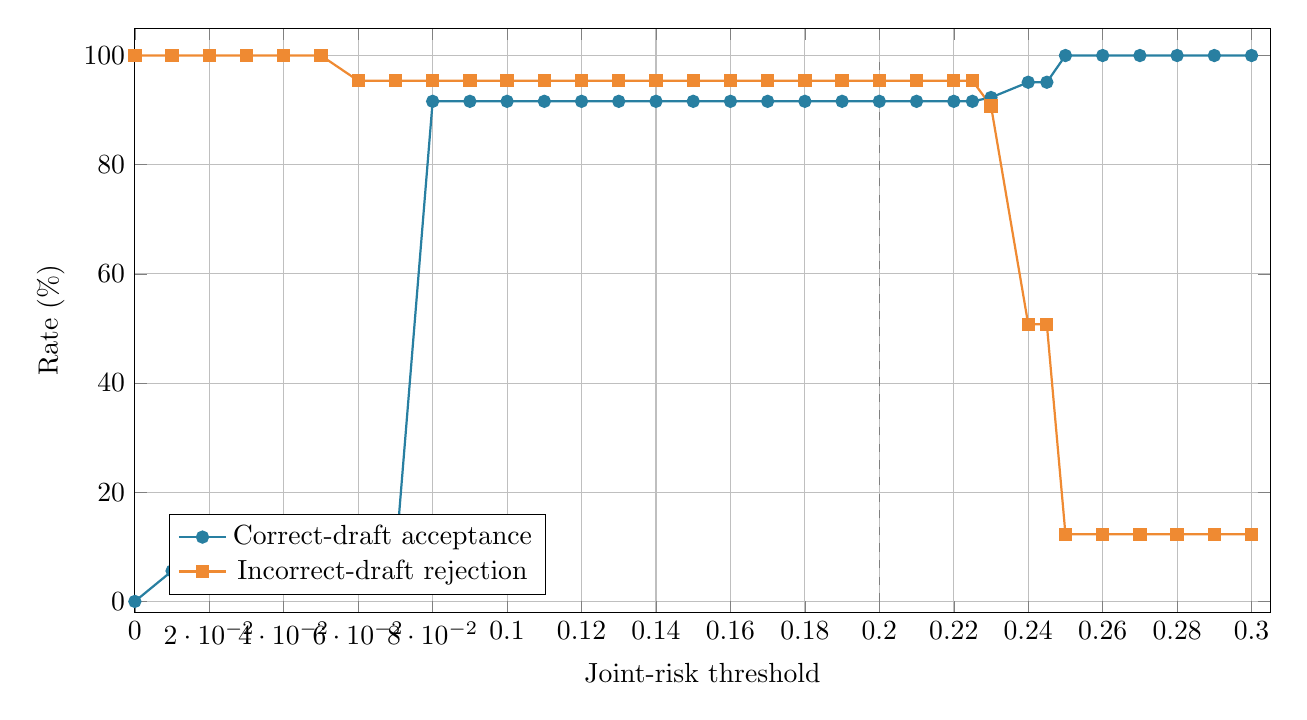
\begin{tikzpicture}\begin{axis}[width=16cm,height=9cm,xmin=0,xmax=.305,ymin=-2,ymax=105,
xlabel={Joint-risk threshold},ylabel={Rate (\%)},grid=major,legend pos=south west]
\addplot[thick,color=curveblue,mark=*] coordinates {(0.0,0.00000000) (0.01,5.59440559) (0.02,5.59440559) (0.03,5.59440559) (0.04,5.59440559) (0.05,5.59440559) (0.06,7.69230769) (0.07,7.69230769) (0.08,91.60839161) (0.09,91.60839161) (0.1,91.60839161) (0.11,91.60839161) (0.12,91.60839161) (0.13,91.60839161) (0.14,91.60839161) (0.15,91.60839161) (0.16,91.60839161) (0.17,91.60839161) (0.18,91.60839161) (0.19,91.60839161) (0.2,91.60839161) (0.21,91.60839161) (0.22,91.60839161) (0.225,91.60839161) (0.23,92.30769231) (0.24,95.10489510) (0.245,95.10489510) (0.25,100.00000000) (0.26,100.00000000) (0.27,100.00000000) (0.28,100.00000000) (0.29,100.00000000) (0.3,100.00000000)};\addlegendentry{Correct-draft acceptance}
\addplot[thick,color=curveorange,mark=square*] coordinates {(0.0,100.00000000) (0.01,100.00000000) (0.02,100.00000000) (0.03,100.00000000) (0.04,100.00000000) (0.05,100.00000000) (0.06,95.38461538) (0.07,95.38461538) (0.08,95.38461538) (0.09,95.38461538) (0.1,95.38461538) (0.11,95.38461538) (0.12,95.38461538) (0.13,95.38461538) (0.14,95.38461538) (0.15,95.38461538) (0.16,95.38461538) (0.17,95.38461538) (0.18,95.38461538) (0.19,95.38461538) (0.2,95.38461538) (0.21,95.38461538) (0.22,95.38461538) (0.225,95.38461538) (0.23,90.76923077) (0.24,50.76923077) (0.245,50.76923077) (0.25,12.30769231) (0.26,12.30769231) (0.27,12.30769231) (0.28,12.30769231) (0.29,12.30769231) (0.3,12.30769231)};\addlegendentry{Incorrect-draft rejection}
\addplot[dashed,gray,forget plot] coordinates {(.2,0) (.2,100)};
\end{axis}\end{tikzpicture}
\caption{联合风险阈值的准入层敏感性分析。对固定 104 个任务的干净／攻击配对场景，共 208 个初始草稿，保持动作、证据、半空间约束及场景风险输入不变，仅改变联合风险阈值。依据独立的批准参数标注，其中 143 个草稿参数正确、65 个参数错误；正确参数放行率和错误参数拦截率分别在这两组内计算。默认阈值 0.20 时，两者分别为 91.6\% 和 95.4\%；在 0.10–0.225 的所测阈值点上结果相同。这是首次提交前的离线准入诊断，未重跑代理的后续核验与恢复，指标不等同于 CU、UA 或 ASR；风险输入沿用原合成场景的声明值。}
\end{figure}\end{document}
